\documentclass{hehe}
\usepackage[utf8]{inputenc}
\usepackage{longtable}
\usepackage{blindtext,alltt}
\usepackage{tikz}
\usepackage{pgfplots}
\pgfplotsset{compat=1.17}
\usepackage{amssymb}
\usepackage{amsmath}
\usepackage{mathtools}
\usepackage{indentfirst}
\usepackage{footnote}
\makesavenoteenv{tabular}
\makesavenoteenv{table}
\usepackage[hidelinks]{hyperref}
\usepackage[nameinlink,noabbrev]{cleveref}
\usepackage{multirow}
\usepackage{makecell}
\usepackage[stype=amc,natbib=true,backend=biber,maxbibnames=20]{biblatex}

\usetikzlibrary{arrows,decorations.markings}

\tikzstyle{basic} = [rectangle, minimum width=3cm, minimum height=0.75cm, text width=2.8cm, text centered, draw=black, fill=white]
\tikzstyle{ios} = [rectangle, minimum width=3cm, minimum height=0.75cm, text width=2.8cm, text centered, draw=black, fill=green!30]
\tikzstyle{ioe} = [rectangle, minimum width=3cm, minimum height=0.75cm, text width=2.8cm, text centered, draw=black, fill=red!30]

\makeatletter
\DeclareRobustCommand\bigop[2][1]{%
  \mathop{\vphantom{\sum}\mathpalette\bigop@{{#1}{#2}}}\slimits@
}
\newcommand{\bigop@}[2]{\bigop@@#1#2}
\newcommand{\bigop@@}[3]{%
  \vcenter{%
    \sbox\z@{$#1\sum$}%
    \hbox{\resizebox{\ifx#1\displaystyle#2\fi\dimexpr\ht\z@+\dp\z@}{!}{$\m@th#3$}}%
  }%
}
\makeatother


\newcommand{\XORsum}{\DOTSB\bigop[0.92]{\Xi}}

%% Full title
\title{File Compression Through Successive Bit Shifted XOR Functions}

%% Shorter title, for use in page header
\runningtitle{SBX File Compression}
\author{Rosie Bartlett}

%% The .bib file containing reference entires, for use with biblatex. CUP-INO loads the biblatex-chicago package with customisations for INO.
\addbibresource{refs.bib}

\begin{document}

\maketitle

\begin{abstract}
Compression is undoubtedly an exceptionally important part of data storage. Throughout this paper I will be exploring a new compression method that utilises XOR functions and bit shifting to compress data.
\end{abstract}

\section{Preface}

To preface this paper, I would like to first explain the notation used throughout this paper. The method being discussed throught this paper is refered to as SBX, for successive bit shifted XOR compression. SBX uses bit shifting to compress correction keys into shorter keys and bit shift lists, or BSLs, which are simply lists of integers. Since there are multiple BSLs, the BSL related to file $n$ will be refered to as $s_n$, where the $i$\textsuperscript{th} value, starting from 1, is refered to as $s_{n,i}$. One of the measures used is in relation to the length of all of the BSLs for a given set of files. In this instance, $s$ refers to all BSLs for the given set of files. Within the scope of this paper, SBX was tested on small amounts of data, and not actual files. For this reason, the term \textit{binary string} is used throughout the paper. This can be seen as equivalent to the term \textit{file}, but in reality it's generation is purely random, unlike a genuine file. The term \textit{pair} is used extensively throughout and refers to a BSL calculation class and key class, and not the actual values contained ithin the classes. For mathematical notation, see \cref{tab:notationTable}.

\begin{table}[ht]
    \centering
    \begin{tabular}{c >{\raggedleft\arraybackslash}p{5.5cm} >{\raggedleft\arraybackslash}p{3cm}}
        \hline
        Symbol & Description & Type \\
        \Xhline{3\arrayrulewidth}
        $s_n$ & Bit shift list for file $n$ & List of integers \\
        $k_n$ & The associated key for file $n$ & Bit string \\
        $D(k_n,s_n)$ & Decoding function. See \cref{eqn:decodeFunc} & Function \\
        $\XORsum$ & Bitwise XOR shorthand. See \cref{eqn:xorsum} & Operation \\
        $<<$ & Bit shift left & Operation \\
        $I_n$ & Correction key. See \cref{eqn:intermediate} & Bit string \\
        $F_n$ & File $n$, where n$\neq0$ & Bit string \\
        $F_{0C}$ & Calculated $F_0$ for a given key and BSL pairing. This may be an incorrect $F_0$ & Bit
        string \\
        $F_0$ & Compressed file & Bit string \\
        $L(s)$ & Number of items in all bit shift strings & Integer\\
        \hline
    \end{tabular}
    \caption{Notation used throughout this paper, in order of occurrence}
    \label{tab:notationTable}
\end{table}

\section{Compression}

\begin{figure}[h!]
  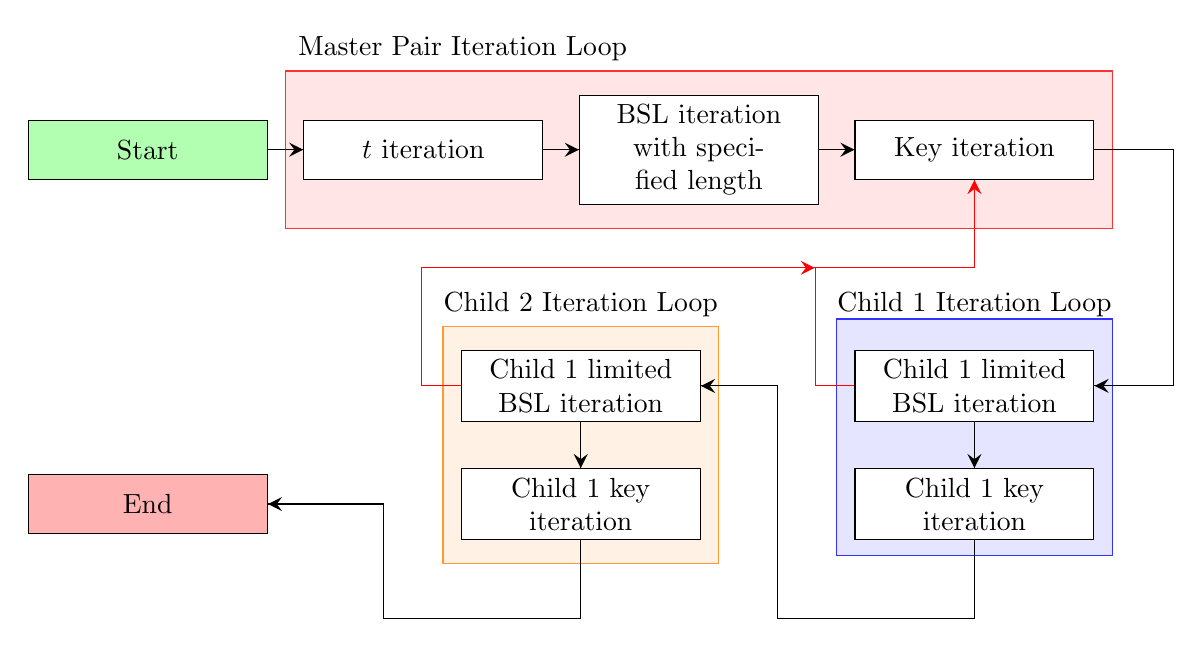
\begin{tikzpicture}[node distance=1.5cm]
    \tikzset{myptr/.style={decoration={markings,mark=at position 1 with %
    {\arrow[scale=1.6,>=stealth]{>}}},postaction={decorate}}}
    \node[above] at (0.5,1){Master Pair Iteration Loop};
    \fill[draw=red!80, fill=red!10] (-1.75,-1) rectangle  +(10.5,2);
    \node (length_iter) [basic] {$t$ iteration};
    \node (Start) [ios, left of=length_iter, xshift=-2cm] {Start};
    \node (bsl_iter) [basic, right of=length_iter, xshift=2cm] {BSL iteration with specified length};
    \node (key_iter) [basic, right of=bsl_iter, xshift=2cm] {Key iteration};

    \node[above] at (7,-2.25){Child 1 Iteration Loop};
    \fill[draw=blue!80, fill=blue!10] (5.25,-2.15) rectangle  +(3.5,-3);
    \node (child1_bsl_iter) [basic, below of=key_iter, yshift=-1.5cm] {Child 1 limited BSL iteration};
    \node (child1_key_iter) [basic, below of=child1_bsl_iter] {Child 1 key iteration};

    \node[above] at (2,-2.25){Child 2 Iteration Loop};
    \fill[draw=orange!80, fill=orange!10] (0.25,-2.25) rectangle  +(3.5,-3);
    \node (child2_bsl_iter) [basic, left of=child1_bsl_iter, xshift=-3.5cm] {Child 1 limited BSL iteration};
    \node (child2_key_iter) [basic, below of=child2_bsl_iter] {Child 1 key iteration};

    \node (End) [ioe, left of=child2_key_iter, xshift=-4cm] {End};

    \draw[myptr] (Start.east) -- (length_iter.west);
    \draw[myptr] (length_iter.east) -- (bsl_iter.west);
    \draw[myptr] (bsl_iter.east) -- (key_iter.west);

    \draw[myptr] (key_iter.east) -| ++(1cm,0) |- (child1_bsl_iter.east);
    \draw[myptr] (child1_bsl_iter.south) -- (child1_key_iter.north);
    \draw[myptr, color=red] (child1_bsl_iter.west) -| ++(-0.5cm,0) |- ++(0,1.5cm) node[anchor=west] (point) {} -| (key_iter.south);
    \draw[myptr] (child1_key_iter.south) |- ++(0,-1cm) -| ++(-2.5cm,0) |- (child2_bsl_iter.east);

    \draw[myptr] (child2_bsl_iter.south) -- (child2_key_iter.north);
    \draw[myptr, color=red] (child2_bsl_iter.west) -| ++(-0.5cm,0) |- ++(0,1.5cm) -- (point);
    \draw[myptr] (child2_key_iter.south) |- ++(0,-1cm) -| ++(-2.5cm,0) |- (End.east);
  \end{tikzpicture}
  \caption{File compression method for three files excluding preprocessing}
  \label{fig:comp_flowchart}
\end{figure}

SBX uses a parallel iterative process to compress files. This process (see figure the one with the flowchart but a better flowchart) is only run once per set of files and returns the optimal BSL for the respective file. This process is in two parts, the first being preprocessing where files are not considered, and the second being file compression. The entire method is outlined in \cref{fig:comp_flowchart}. Please note however, that each node is representative of an iterative loop, that when ended returns to the previous node. For the child BSL iteration nodes however, once these have ended, they return to the master pair key iteration node.

\subsection{Proprocessing}

Before any of the files are even considered, a small amount of preprocessing must be performed. This preprocessing consists of populating two empty lists, which will be referred to as $s_0$ and $t$. The first list to be populated, $s_0$, is an exhaustive list of all the possible BSL values. When this list is being populated, teach item added to it is an exhaustive list of BSL values of a specific length, with this length starting at one and ending with a length of $l$. The second list, $t$, is all the different combinations of BSL value lengths for all the different files. This is ordered in ascending order where the value being considered is the sum of each value within $t$.

For example, when $n$ is 2 and $l$ is 3, the first list, $s_0$ would be \texttt{[[[0], [1], [2]], [[0, 1], [0, 2], [1, 2]], [[0, 1, 2]]]}, and the $t$ would be \texttt{[[1, 1], [2, 1], [1, 2], [3, 1], [2, 2], [1, 3], [3, 2], [2, 3], [3, 3]]}.

Once this has been completed, the files can now be considered. This consists of the files being allocated to classes that all hold their respective file. The first file is different to the others, as it is held by a master pair class instance which controls all of the compression. Each class contains more data needed for the compression such as the key length, and references to the master pair node class instance for the child nodes, and a list of references to the child nodes for the master pair node.

\subsection{File Compression}

Once the preprocessing has finished, then the compression can begin. The compression is controlled by the master pair node, and begins begins by iterating over each of the items in t. For each of these, it iterates over each of the possible BSL values with a length specified by the first item in the current iteration of t. For each of these iterations, every possible value for the key is iterated over and $F_{0c}$ is calculated, see \cref{eqn:f0c}, using the current value of the BSL and the current value of the key.

\begin{equation}\label{eqn:f0c}
  F_{0c}=k_1\oplus s_1
\end{equation}
\begin{equation}\label{eqn:in}
  I_n=F_n\oplus F_{0c}
\end{equation}

Once $F_{0c}$ has been calculated, the master pair begins iterating over each of the child nodes. For each child node iteration, a small amount of preprocessing must be performed first to enable checks later on. This preprocessing contains calculating $I_n$, and then the offset of the first and last non-zero bit in $I_n$. Once these have been calculated, the child begins iterating over all possible BSL values with a length specified in the current iteration of $t$ in the master class. The index of the child within the master pair class' list of children is the index used in retrieving the current BSL length to iterate over, with the first child accessing the second item in the current iteration of $t$, the first value being already used for the master pair class.

It is here that the first efficiency check is performed. The first value in the current BSL value has to be less than or equal to the index of the first non-zero bit in $I_n$, and the last value in the current BSL added to the length of the key must be larger than or equal to the index of the last non-zero bit in $I_n$. This check ensures the the current BSL is able to produce a non-zero bit in the lowest and highest index required. If this check is passed, then the child node then attempts to calculate a key that, when paired with the respective BSL, would result in $I_n$. This calculation is performed bitwise, calculating the required bit needed to produce the relevant bit in $I_n$. This calculation has to be performed bitwise since each successive step requires the previous bits to have been calculated. However, this calculation method is not perfect and errors can be introduced throughout. Because of this, once the key calculation has been performed, the result of the calculation is passed into the key expansion method, along with the respective BSL, the result of which is compared against $I_n$. If these are identical then the child returns true to the master pair node, which then continues iterating over the remaining children. If none of the child BSL values could be used, then a new key is generated and the process begins again. Once all children have successfully been iterated over, the master pair and all child nodes save their values and the iterative process is ended. This can be done due to the sorting of $t$ in the preprocessing. Since t was sorted by the sum of each of the elements, then once all children have successfully been iterated over, then there cannot be a shorter values of $L(s)$ for the current set of files, and so iteration is ended.

\section{Expansion}

\section{Results}

To evaluate the effectiveness of SBX, it was run on several different sets of data, each set having a different batch and file size. The code was run on a three node raspberry pi cluster, appendix time me thinks for detailed specs, and times for each compression have been included. Each set of data contained 1000 pseudo-randomly generated files.

\section{Future Work}



%% Optional appendix
\appendix
\section{Raspberry Pi Cluster Specifications}
This appendix details the specifications of the Raspberry Pi cluster that SBX was tested upon.

\begin{itemize}
  \item \textbf{Master Node}:\\
  \begin{itemize}
    \item Raspberry Pi model B
    \item Something else?
  \end{itemize}
\end{itemize}



\printbibliography

\section*{Author}
\begin{authorbio}

\textbf{Rosie Bartlett} is a currently a student and is still developing SBX. She can be reached at abc@xyz.edu. GitHub is also a good way to keep up with the current version of SBX.
\end{authorbio}

\section*{Acknowledgements}
I would like to thank

\section*{Key Words}
Keyword one; keyword two; keyword three; keyword four.

\end{document}
